\documentclass[conference]{IEEEtran}
\usepackage{verbatim}
\usepackage{cite}
\usepackage{graphicx}
\usepackage{amsmath}
\usepackage{amssymb}
\usepackage{amsthm}
\usepackage{mathtools}
\usepackage{color}
\usepackage{multirow}
\usepackage{array}
\title{\author{Micah Thornton, Fanchen Zhang, Jennifer Dworak} Intelligent Targeting of Cell-Aware Type 
Faults Using Mandatory Conditions for Fault Detection}
\newcommand\MyBox[2]{
  \fbox{\lower0.75cm
    \vbox to 1.7cm{\vfil
      \hbox to 1.7cm{\hfil\parbox{1.4cm}{#1\\#2}\hfil}
      \vfil}%
  }%
}
\begin{document}
\maketitle{}
\begin{abstract}
        \begin{comment}

    This paper outlines our current progress in the search for intelligent targeting methods for a class of faults known as ``Cell-Aware Type Faults''. We begin with a brief introduction to cell-aware faults and a description of how they differ from the cell-aware type faults that we are examining in this endeavor. We then describe our over-arching research goal: To find an attribute that can predict whether or not cell-aware faults can cause serious problems during functional usage. We then present our research methodology beginning with the generation of a describing-fault-model for cell-aware type faults, and an analysis of potential attributes that can be used to classify and characterize cell-aware type faults. Our findings are discussed, and the respective benefits to manufacturing test are discussed.


    \end{comment}

    The ``Cell-Aware'' fault model does an excellent job of expressing potential in-gate defects. Unfortunately some circuits contain too many potential cell-aware faults to test for with the limited resources available to test engineers. To avoid detailed analog modeling, and fault extraction we modeled cell-aware faults using a methodology wherein stuck-at ATPG was the primary fault modeling procedure used.  We differentiate these faults from their analog counterparts by deeming them ``Cell-Aware-\textit{Type}'' faults
    To determine the most important faults to target, we extracted the ``mandatory conditions'' for detection for each potential fault in two test circuits, and performed functional simulation to determine how many times these mandatory conditions were met.
    We then analyzed the correlation between mandatory condition counts for faults, and the corresponding faults detection during goodstate simulation. 
    Our results include the discovery that mandatory conditions are a good predictor of a fault's relative importance in a circuit whose intended function is known, provided that the potential state space is sufficiently explored during functional operation. 
\end{abstract}
\section{Introduction}
    \label{sec:intr}
        A primary concern in test is the limited resources available to test engineers. 
    These constraints severely limit the breadth of IC test. 
    Most circuits are only tested over a brief period of time or with limited computational resources. 
    Granted, if resources were unlimited we would want to test for every possible manufacturing defect.
    Unfortunately, resources are scarce in any industry, and especially so in the circuit design world. 
    Even with unlimited resources, if an average-sized circuit were tested for every possible fault, it could take longer than the known age of the universe to finish. 
    We would finally be able to present a tested product and then the universe would collapse on itself. 
    Because of these limitations, it becomes necessary to shrink the test space to a reasonable size. 
    The work detailed in this paper discusses how cell-aware test-space minimizing decisions can be made during functional simulation.


    Fault models are used as aids by test engineers to describe possible defects in a circuit and to generate input patterns to test for them. 
    One of the more predominantly used fault models is known as the ``Stuck-At Fault Model.''
    In this model, wires are modeled as being stuck at logic value-1 (\textit{shorted to $V_{dd}$}) or logic value-0 (\textit{shorted to ground}).
    One essential fact about this model, is that defects occur on the lines between gates,  not within them. 
    For example, to represent a potential stuck-at fault, the top wire in Figure \ref{fig:safault} is stuck-at 0 and is therefore \textit{modeled} as being grounded.

    \begin{figure}[h!]
        \begin{center}
            \caption{Example of Stuck-At Fault}
            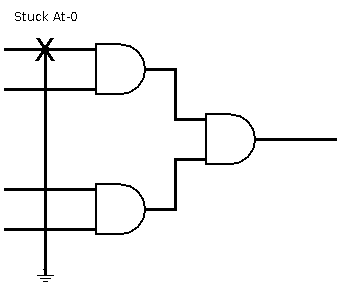
\includegraphics[scale=0.5]{Figures/sa0.png}
            \label{fig:safault}
        \end{center}
    \end{figure}

    This particular fault will cause major problems because the output of the circuit evaluates to 0 without regard to any other inputs. 
    Note that, in this case, the defect is described and conceptualized as a problem within the boundary between primary inputs and the gate, rather than occurring within the gate itself.


    To test for any fault you must first excite the fault and then observe the output.
    In this case we would need to make certain that the first PI (Primary Input) was set to 1 in order to excite the fault.
    We would also need to ensure that the fault will propagate to the output of the entire circuit. 
    For this particular fault, only one pattern will excite the fault and allow propagation to the output (\textit{inputs = 1111}). 
    Generally an ATPG (Automatic Test Pattern Generation) tool is used to create a list of possible patterns that could detect a fault.
    In this research we used both stuck-at fault ATPG and ATPG on a UDFM (User Defined Fault model, defining cell-aware type faults), by taking advantage of a built-in feature of Mentor Graphic's Tessent. 

    For the research in this paper, we consider a fault model known as the ``Cell-Aware Fault Model.''
    This fault model considers the transistor arrays within a logic gate and is explained in more detail with an example in section \ref{sec:caf}.
    The focus of this research is to determine a method for assigning an ``importance attribute'' to each of the cell-aware faults. 
    In other words, because we cannot focus on all potential cell-aware faults, how can we decide which ones present the most obvious flaws during normal usage? 
    To make this determination we propose using an attribute of a cell-aware fault called ``Mandatory Conditions'' during functional simulation to rank faults. 
    Functional simulation will be discussed in more detail in Section \ref{sec:fs}.
    The way that we performed functional simulation will be discussed in Section \ref{sec:meth}.
    Results and analysis will be discussed in Sections \ref{sec:res}.

\begin{comment}


    The abstract concept of a cell-aware fault is best described as any fault that is caused by a certain defect within a standard cell. Meaning that the fault specifically models a problem within the transistor array of the cell. Because this describes exactly every defect from manufacturing view, the fault model can be thought of more effectively as a model that represents faults that cannot be explained by some other traditional fault model such as the stuck at or bridging fault model. The cell-aware model and it's testing framework as well as ATPG methods were introduced by Hapke et al. \cite{5355741} \cite{Hapke} \cite{6401533}. The cell-aware fault model pays particular attention to the contents of the standard cell library which is used in the design of a circuit. The promise of using this fault model was explored in more detail by Rajski et al. \cite{5227030}. The effectiveness of the cell-aware fault model for detecting faults, and a comparison to the small delay defect fault model was explored by Fan Yang et al. \cite{6979084}. A case study regarding the usefulness of the cell-aware fault model on diagnosing a micro-controller was done by Prabhu et al. \cite{6847826}.

    In conjunction with the research discussed in this paper we discovered that n-detect for forcing multiple detections in certain ATPG schemes wouldn't work for cell-aware type faults. Consequently the definition of a cell-aware type fault in contrast to a pure cell-aware fault was discussed in a previous paper we wrote. \cite{6875445} The difference between what we have been referring to as a cell-aware type fault and a pure cell-aware fault arises in the derivation of each. As above mentioned, the cell-aware fault model can be viewed two ways that are essentially the same. The first is as an internal defect something tangible within the transistor array, Cell-aware faults can be derived by examining the electrical connections, and relationships. The second is as a fault that cannot be described by another fault model, and would thus not be tested for in ATPG targeting a specific type of fault. viewing the cell-aware fault by this second means is simply not the standard meaning for one, and we have hence taken to referring to them as cell-aware type faults. The definition of, and creation of the cell-aware type fault model is where the discussion of our methodology begins.

\end{comment}

\section{Previous Work}
    \label{sec:pw}
    \begin{comment}


    The abstract concept of a cell-aware fault is best described as any fault that is caused by a certain defect within a standard cell. Meaning that the fault specifically models a problem within the transistor array of the cell. Because this describes exactly every defect from manufacturing view, the fault model can be thought of more effectively as a model that represents faults that cannot be explained by some other traditional fault model such as the stuck at or bridging fault model. The cell-aware model and it's testing framework as well as ATPG methods were introduced by Hapke et al. \cite{5355741} \cite{Hapke} \cite{6401533}. The cell-aware fault model pays particular attention to the contents of the standard cell library which is used in the design of a circuit. The promise of using this fault model was explored in more detail by Rajski et al. \cite{5227030}. The effectiveness of the cell-aware fault model for detecting faults, and a comparison to the small delay defect fault model was explored by Fan Yang et al. \cite{6979084}. A case study regarding the usefulness of the cell-aware fault model on diagnosing a micro-controller was done by Prabhu et al. \cite{6847826}.

    In conjunction with the research discussed in this paper we discovered that n-detect for forcing multiple detections in certain ATPG schemes wouldn't work for cell-aware type faults. Consequently the definition of a cell-aware type fault in contrast to a pure cell-aware fault was discussed in a previous paper we wrote. \cite{6875445} The difference between what we have been referring to as a cell-aware type fault and a pure cell-aware fault arises in the derivation of each. As above mentioned, the cell-aware fault model can be viewed two ways that are essentially the same. The first is as an internal defect something tangible within the transistor array, Cell-aware faults can be derived by examining the electrical connections, and relationships. The second is as a fault that cannot be described by another fault model, and would thus not be tested for in ATPG targeting a specific type of fault. viewing the cell-aware fault by this second means is simply not the standard meaning for one, and we have hence taken to referring to them as cell-aware type faults. The definition of, and creation of the cell-aware type fault model is where the discussion of our methodology begins.

\end{comment}
The cell-aware fault model is central to this research. 
To place it in context, we begin with a discussion of its history. 
The cell-aware fault model and its testing framework were defined by Hapke et al. \cite{5355741}, although previous work along the same lines was done by Sharma et al.\cite{4437604}. 
Hapke has done further work with the model by creating a tutorial for its use in industry\cite{Hapke}, applying it to a 32-nm laptop processor in a case study\cite{6401533},  applying it to automotive parts in another case study\cite{6847814}, creating a new testing procedure for it \cite{6879635}, showing industrial results \cite{5783604}, and extending it to allow for detection of some internal small delay defects\cite{6139151}. 
Fan Yang et al. compared results from the use of both the cell-aware and small delay defect fault model in \cite{6979084}.

The method by which we perform functional simulation was first proposed as a way to determine fault coverage information at ITC in 2011 by Shi et. al\cite{6139146}. 
This work itself was an extension of an earlier paper that described targeting very difficult stuck-at faults\cite{4700614}. 
Our research is different from this previous work due to the use of the cell-aware fault model and the non-exclusive targeting of only hard stuck-at faults.
On the contrary, in this research many faults may be easy to detect.

 Previously we have shown that some cell-aware-type faults are resistant to n-detect, especially when a test set is optimized for multiple detections of stuck at faults with few patterns. 
 In the same paper, we discussed using cell-aware-type top-off patterns as a means to prioritize cell-aware-type faults when testing resources are limited.\cite{6875445}. 


\section{Cell-Aware Type Faults}
    \label{sec:caf}
    In this research the primary fault model of concern is the ``cell-aware fault model.''
To differentiate this from other types of fault models, consider the locations at which faults can occur. 
For instance, consider the example of a stuck-at fault in Section \ref{sec:intr}.
As was stated there, a stuck at fault can only occur on the interconnects between logic gates. 
Perhaps a more technically correct way of saying this is: defects can only be modeled as occurring on logic nets. 
As another example, examine Figure \ref{fig:bf} which represents a couple potential faults using the bridging fault model.

\begin{figure}[h!]
\centering
\caption{Example of a Bridging Fault\label{fig:bf}}
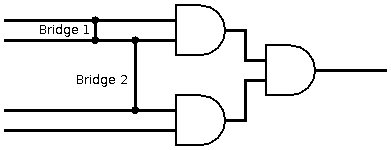
\includegraphics[scale=0.5]{Figures/bf.png}
\end{figure}  

Notice again that the faults in this example occur on electrical nets outside of the logic cells. 
To extend the analogy, these types of fault models could be labeled as ``cell-unaware faults.''
This is because the defects are all modeled without respect to the internals of each of the standard cells in the circuit. 
This is not to say that faults can only occur outside the gates.
Many faults occur within logic cells, but are able to be effectively modeled and detected by fault models which represent faults outside standard cells. 
In other words, even though the manufacturing defect doesn't produce a circuit exactly like the one seen in Figures \ref{fig:safault} and \ref{fig:bf}, these faults can be effectively modeled as and tested for by thinking of the circuit as shown. 

Unfortunately, the disregard for the internals of a standard cell produce a large class of faults which will not be considered. 
Or rather, will not be targeted during ATPG for a fault model that only considers the electrical nets between gates.
To get a better feel for cell-aware type faults we will perform cell-aware type ATPG for the NOR gate in Figure \ref{fig:nor}. 
To discover the internal faults that will not be tested for by a traditional fault model, we will first perform ATPG with regards to the traditional model.
For this example (and in this research) we use the stuck-at fault model.

\begin{figure}[h!]
\centering
\caption{Nor gate for stuck-at ATPG Example\label{fig:nor}}
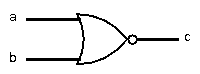
\includegraphics[scale=0.5]{Figures/nor.png}
\end{figure}
\begin{center}
\begin{tabular}{ c c | c }
    a&b&c \\
    \hline
    0&0&1 \\
    0&1&0 \\
    1&0&0 \\
    1&1&0 \\
\end{tabular}
\end{center}

There are six potential stuck-at faults that we need to test for: a stuck-at 0, a stuck-at 1, b stuck-at 0, b stuck-at 1, c stuck-at 0, and c stuck-at 1. 
To derive the stuck at test set, let us find the smallest set of patterns that will test for each of these faults. 
To test for a fault, we must first excite the fault, and then observe the net at the output of the circuit ( This is done with the use of the Boolean derivative). 
To excite a fault, we force a net to the opposite value than what it is stuck at. 


\begin{align*}
    T_{a/0} &= a\frac{\delta a}{\delta c} = a\overline{b} \\
    T_{a/1} &= \overline{a}\frac{\delta a}{\delta c} = \overline{a}\overline{b} \\
    T_{b/0} &= b\frac{\delta b}{\delta c} = b\overline{a} \\ 
    T_{b/1} &= \overline{b}\frac{\delta b}{\delta c} = \overline{b}\overline{a} \\ 
    T_{c/0} &= \overline{a}\overline{b}\frac{\delta c}{\delta c} = \overline{a}\overline{b} \\ 
    T_{c/1} &= (\overline{a}b + a\overline{b} + ab)\frac{\delta c}{\delta c} = (\overline{a}b + a\overline{b} + ab) 
\end{align*}

To minimize the test set, the ATPG tool would then na\"ively suggest:

\begin{equation}
T=\{a\overline{b}, \overline{a}b, \overline{a}\overline{b}\}
\end{equation}

With this test set, we can effectively test for all stuck-at faults in our small example circuit. 
But we are simply \textit{modeling} faults as occurring on lines outside of logic gates.
What if the real fault is inside the circuit, and can only be detected with the test pattern $ab$ (or a = 1 and b =1)? 
Figure \ref{fig:caf} illustrates a cell aware fault inside a nor gate, and describes the test pattern that detects it. 

\begin{figure}[h!]
\centering
\caption{Example of a Cell-Aware Fault\label{fig:caf}}
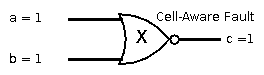
\includegraphics[scale=0.5]{Figures/caf.png}
\end{figure}  

A good understanding of the cell-aware fault model is essential for understanding parts of our methodology.
This example is a good introduction to cell-aware faults.
Ron Press posted an excellent tutorial explaining these faults online in 2012\cite{ronpress}.
\section{Functional Simulation}
    \label{sec:fs}
    Circuit simulation can be performed at different levels of abstraction. 
Behavioral simulation is the highest level of abstraction and functional simulation is the next highest. 
Technically, the only difference between behavioral and functional simulation is the inclusion of unit-delays within the circuit for functional. 
The addition of unit delays for cells in the simulated circuit allows for the comparison of ``theoretical delays'' among different circuits. 
Behavioral or functional simulation is used to used in industry to verify that a circuit is meeting its intended function. 
During functional simulation, functional test patterns are supplied to a circuit, and circuit output responses are monitored to ensure that the circuit is functioning as intended. 
This can be done in several different ways, but the goal is to supply meaningful inputs to the circuit, and observe meaningful outputs. 


Consider any generic processor.
If the processor receives an instruction that does not contain a valid op-code, it will be put into an unknown op-code state. 
In order to test this processor for defects, we would like to supply it with instructions that test all of the internal circuitry. 
Supplying it with one unknown opcode would test certain parts of the exception handling routines, but we shouldn't supply the processor with \textit{only} instructions that have unknown opcodes.
If we did, we would not be able to effectively test the rest of the circuitry. 
Supplying a circuit with many different inputs to test all of the corner cases of the state space is the goal of proper functional verification. 


Consider Figure \ref{fig:sd1}. 
This diagram represents the state space of a fabricated circuit. 
We call $S$ the set of all possible ``Circuit goodstates.''
The size of the $S$ is equivalent to $2^{m}$, where $m$ is the number of memory elements the circuit.  
Assume there are three known functions of the circuit: $A, B,$ and $C$. 
These functions are known to use subsets of the states in $S$, denoted by $S_{A}, S_{B},$ and $S_{C}$ respectively.
During manufacture a defect was introduced to the circuit. 
This defect can only be detected if the circuit is operating in a state in goodstate grouping denoted $F$.


\begin{figure}[h!]
\centering
\caption{Arbitrary State Space\label{fig:sd1}}
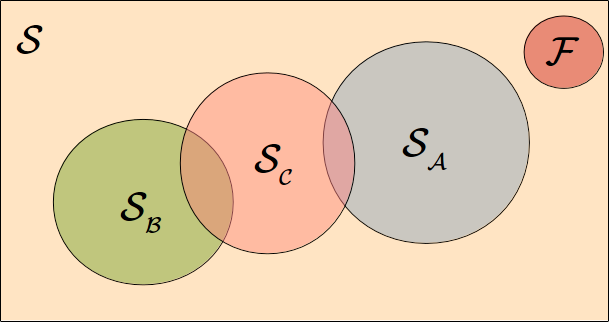
\includegraphics[scale=0.5]{Figures/sd1.png}
\end{figure} 

Fortunately, this fault does not conflict with any of the three known functions state spaces.
Imagine that a customer was only going to use functions $A, B,$ and $C$.
They would never experience the fault, because they never operate the circuit in a state space that overlaps with it. 
This means that there would be absolutely no reason to discard this circuit, because it would still be useful to the customer. 
By performing this sort of functional simulation of circuits, we can rate faults in terms of how many times they might be encountered during functional use.
Using functional simulation as well as a few additional parameters to rate these faults in terms of their general importance allows  more efficient resource allocation. 
This resource allocation is the primary purpose of this research. 
\section{Research Methodology \& Experiment}
    \label{sec:meth}
        \begin{comment}
    In order to describe the input and output combinations that would indicate a cell-aware fault occurred, we created something called a user defined fault model (UDFM). The generation of the UDFM itself was simple, the most difficult task came about when selecting possible input-output combinations that would indicate a cell-aware fault. We choose to select these combinations based on the key fact that cell-aware type faults are resistant to stuck-at ATPG. We took the standard cell library for which we were to generate the UDFM, and then created small verilog modules to describe each of the standard cells, and then performed stuck-at ATPG on these verilog modules. We then examined the pattern files that were generated and selected input combinations that would conflict with the truth table of the standard cell, and would also not be tested for by stuck at ATPG, and inserted them into the UDFM. 


    Targeting all of the possible cell-aware faults is costly, and impossible in most cases. There are a specific sub-class of cell aware faults that will affect the devices output or function during normal usage. The point of our study was to find an effective manor in which this sub-class can be specifically targeted by an ATPG tool. In short, when resources are limited we may only want to focus on faults that are especially likely to cause field errors, or functional faults. 



    To try and discover a methodology whereby the prediction of functional faults becomes a systematic process we had previously extracted circuit goodstate patterns. The premise was that by extracting these goodstates we have a list of possible states that the circuit can be in during functional usage. The goodstate patterns that were extracted included the contents of every state cell (i.e. flip flops and latches) for the circuit. Initially we used five ISCAS 1989 benchmark circuits, unfortunately it was very difficult to discover and provide functional inputs to the circuits. We instead generated a couple random input patterns for each of the five circuit that we were using. We then allowed the circuits to update for 40,000 clock cycles, and captured the contents of all the memory elements in the circuit after every clock cycle. Our thoughts were that no matter what the circuits function was, and no matter the inputs that it received, we could expect state values that would result during functional usage. 

    Because capturing these goodstates is expensive memory wise, we proceeded to think of ways that a similar analysis could be done during functional simulation. This would allow us to predict which faults would be most likely to cause errors during functional usage simultaneously, without having to store off goodstates and then reuse them. 

    We began this analysis by using ATPG on the faults described in the UDFM that we created earlier. This allowed us to see which state bits and inputs were mandatory for our cell-aware faults to be detected. Due to the nature of a test pattern propagating the fault to the output, it was evident that the test patterns generated would indeed see the faulty circuit values propagated to the outputs of the circuit. This means that if these patterns were to occur, then the fault would cause problems during the functional usage of the circuit. Because multiple patterns were generated for each of the faults that we described in the UDFM, it was possible to examine the the state bits, and input bits which didn't change for each input pattern, and to determine the bits that were set or reset in every pattern that detected the fault. These bits being either set or reset depending on the fault are a particular attribute of the circuit, and are called the mandatory conditions for fault detection or simply the mandatory conditions. 

    For example, imagine a small 4 input circuit with few gates. Imagine that we performed stuck-at ATPG on the circuit and in order to detect one of the stuck-at-0 faults the following 3 input patterns were given: 0010, 0110, 0111. In all three cases the first input bit is reset and the third is set, so the two mandatory conditions for detecting this stuck-at-0 fault are: input\_1 = 0, and input\_3 = 1. We performed this analysis for each of circuits, for each fault in the UDFM, and arrived at a long list of the mandatory conditions required for fault detection.  

    The next step was to monitor how many times the mandatory conditions were all met for each fault during functional simulation(running through each of the sets of goodstates we captured). This meant that we were able to gain a quantifiable value that was indicative of how many times a cell-aware fault would directly affect the output of the circuit. We should now be able to more effectively target only those specific faults that have a much greater bearing on the overall output of the circuit that is produced. 

    There are a few scenarios that are worthy of consideration before the results of this procedure are discussed. The first scenario arises when the total functionality of a circuit is known, and the goodstates that are captured are distributed equally among the state space of the device. In this case, using mandatory condition counts from functional simulation is probably a good indicator as to whether or not such faults should be targeted because the full functionality of the circuit is represented. On the other hand, the test engineers may have to contend with 3rd party IP, and can thus only know some of the total functionality of the circuit. This means that the goodstates they generate for functional simulation will be constrained to a much smaller portion of the entire space state, and in this case other considerations should be made when determining whether or not a fault should be tested for based on its functional application. 

    We are currently investigating a data encryption standard circuit DES56, and are performing a similar analysis to that which was performed on the ISCAS benchmark circuits. The major difference between the previous circuits and this one is that we understand the full functionality and have a working functional testbench for the encryption circuit, whereas it was very difficult to discern the purposes of the ISCAS circuits, and we had to resort to using random input vectors to generate their goodstates. In the analysis section we refer to the number of times that all the mandatory conditions were met for a particular fault during the functional simulation as that fault's ``mandatory count'' 
    \end{comment}

    \subsection{Cell-Aware Type UDFM Generation}
    In Section \ref{sec:caf} several types of faults were discussed, but in particular detail the cell-aware-type fault was introduced. 
    We also showed how to find a potential input vector that could be used to test for a cell-aware-type fault(by a nor-gate example). 
    The input vector, identified for cell-aware-type fault detection, was illustrated in Figure \ref{fig:caf}.
    Note that this represented only a single gate, and not a gate within a circuit. 
    The two circuits on which this analysis was performed are an ISCAS 89' benchmark circuit (s9234) and a DES56 encryption/decryption circuit from opencores.org.
    Each of them were synthesized using a different standard cell-library.
    These libraries included many different types of cells such as And-Or-Inverts, Half-Adders, and Three-Input NORs. 
    It became our task to develop a standard way of finding which patterns could be used to detect the cell-aware-type faults. 
    We did this in a very similar manner to the example in Section \ref{sec:caf}. 
    To automate the process, we used a standard stuck-at ATPG tool (Mentor Graphics Tessent)to generate the stuck-at test patterns so we didn't have to do it manually (as was shown in the example).
    We then cross-referenced each standard cells truth table, and determined what input pattern could be used to detect a fault within that cell. 
    Finally, to define a fault model that fit the input vectors we were generating, we used some built in functionality of the Tessent which allowed us to define our own fault model, a UDFM (User-Defined-Fault-Model).
    After generating a UDFM that properly represented several potential cell-aware-type fault input-output pairings,  we moved on to the next part of the experiment.

    \subsection{Mandatory Condition Extraction}
    To allow for the prediction of the importance of specific cell aware faults in a given circuit, we first had to extract an attribute of each fault individually. 
    As was shown before in section \ref{sec:caf}, certain input vectors are required to test for a given fault. 
    For the cell-aware fault in Figure \ref{fig:caf} only one such input vector was specified. 
    Granted, that circuit is only one gate and as such only one pattern could have potentially detected a cell-aware fault. 
    For larger more realistic circuits that consist of many gates, there are many different patterns that can detect the same fault.

    A certain feature of most ATPG tools called ``n-detect.'' 
    This approach allows for the user to specify a value of n. 
    The specified value is then used as a target for the tool to generate a set of patterns that detect each fault at least n times.
    Specifying a large value of n will return many patterns that detect the same fault in an output file format called a fault dictionary. 
    The fault dictionary is essentially just a cross-listing of patterns and the respective faults they detect. 
    We used a similar method to n-detect to allow for the generation of a fault dictionary, which we then examined to extract a general formula for patterns that could detect a given fault. 
    These formulas are henceforth referred to as the mandatory conditions for fault detection. 


    Imagine a circuit $C$ has a potential cell-aware fault $f$, six primary inputs, labeled: $p_{0}-p_{5}$, and 2 internal state elements (D-Flip-Flops, Latches, etc...), labeled $d_{0}-d_{1}$ from most significant to least significant.
    $C$ is large enough that four test patterns exist that can detect $f$. 
    Assume we set the n-value to some arbitrary number greater than four. 
    After running ATPG, using the UDFM generated above, the following patterns are described in the fault dictionary. 


    \begin{center}
    \begin{tabular}{| c | c | c |}
        \hline
        & Inputs & Flip-Flops\\
        \hline
        \hline
        Pattern 1 & \textcolor{red}{0}1011\textcolor{red}{1} & 0\textcolor{red}{0} \\
        \hline
        Pattern 2 & \textcolor{red}{0}0100\textcolor{red}{1} & 1\textcolor{red}{0} \\
        \hline
        Pattern 3 & \textcolor{red}{0}1111\textcolor{red}{1} & 0\textcolor{red}{0} \\
        \hline
        Pattern 4 & \textcolor{red}{0}0000\textcolor{red}{1} & 1\textcolor{red}{0} \\
        \hline
    \end{tabular}
    \end{center}

    Notice that the values in red do not change at all in any of the patterns, but that ever other bit changes. 
    There are three mandatory conditions, we denote the mandatory conditions of $f$ as $MC(f)$.
    We can now derive $MC(f)$ for this circuit, because we know all of the patterns that detect the fault. 
   
    In general, it is difficult to know how many patterns are capable of detecting a particular fault without exhaustive analysis. 
    Thus it is important that the value of n be selected be appropriately large to help increase the probabiliity that the identified conditions are truly mandatory. 

    \begin{center}
    \begin{Equation}
        $MC(f) = \overline{p_{0}}p_{5}\overline{d_{1}}$
    \end{Equation}
    \end{center}

    The next part of the setup is to count how many times these mandatory conditions are met during functional usage.
    However, we must first discuss how we performed functional simulation. 


    \subsection{Circuit Goodstate Extraction & Functional Simulation}

    For s9234, we did not know the original function of the circuit. 
    We intentionally allowed its intended function to remain obscured so we would only test for a certain small part of the overall state space. 
    This experiment is representative of rating the importance of cell-aware faults for a circuit whose function is unknown, or only one function of a group of many is known.
    This was to emulate a company using an obfuscated circuit of which they only know one intended use.
    We first inserted a scan chain into the circuit in order to allow for the extraction of state bits. 
    We then generated 40,000 random inputs, and extracted the total complement of state bits after each clock cycle. 
    We stored these as the first set of 40,000 goodstates, and then generated another set. 
    Finally we created a test bench which allowed the functional simulation of s9234, using the goodstates.


    For DES56 however, the intended purpose was known. 
    We also had a functional test bench for this circuit already which was used in previous research.
    We used the DES56 circuit to encrypt and decrypt the plain text ASCII version of this paper \cite{1299219}. 
    This qualifies as functional simulation of the circuit because it is realizing the intended purpose of both encryption and decryption. 
    We covered a much higher percentage of the state space during this functional simulation. 
    This was intended to emulate the testing of a circuit whose functionality is known in its entirety. 


    Lastly, we detected the number of times that a faults mandatory conditions were met during functional simulation.
    This was the key attribute that we intended to use for fault importance predictions. 
    We henceforth refer to this value as the ``mandatory count'' for a particular fault.
    This is discussed in the next subsection.
    

    \subsection{Mandatory Counts during Functional Simulation}
    As we have seen, the mandatory conditions for a given fault can be represented as a boolean function of the fault. 
    In the example above we determined that $MC(f) = \overline{p_{0}}p_{5}\overline{d_{1}}$. 
    The result that these mandatory conditions can be represented as a boolean function is essential. 
    By representing them as a boolean function we can add a few simple logic gates with an output signal that feeds a counter. 
    We created a script to read the mandatory conditions file that was created by parsing the fault dictionary. 
    This script output a testbench to allow for functional simulation of the circuit, but it added a few of these extra logic gates that allowed us to keep a count of how many times the mandatory conditions for each fault were met during functional simulation. 
    The logic gate that would be added to the circuits test bench in order to examine whether the mandatory conditions for the fault detailed above is given in Figure \ref{fig:mandgate}

\begin{figure}[h!]
\centering
\caption{Mandatory Condition Detector for fault f\label{fig:mandgate}}
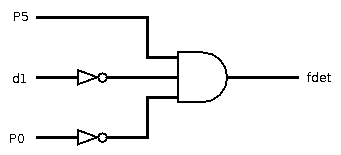
\includegraphics[scale=0.5]{Figures/mand.png}
\end{figure} 

    Because the mandatory conditions were generated based on test patterns that were engineered to propagate the fault to the outputs of the circuit, if they are met during functional simulation, then a device with this fault will output an erroneous value during its use.  
    We can use the mandatory counts for each fault to rank them in terms of their importance.
    They can then be sorted by the probability that they will cause problems during the functional use of the device. 
    In order to determine if the mandatory counts were a good indication of whether or not the fault would be detected during functional use, the last part of the experiment consisted of the use of a fault simulator to determine whether or not a fault would be detected during the same ``goodstates''. 
    We could then set a prediction criteria in terms of the mandatory counts for a particular circuit and construct a confusion matrix and calculate the corresponding statistics to determine how well these mandatory counts predicted whether or not a fault was truly functional (would be detected during fault simulation). 
    
\section{Results \& Analysis}
    \label{sec:res}
    
    \begin{comment}


    To perform an analysis of the results and determine if there was correlation between the number of times the mandatory conditions were met and whether or not we would classify the fault as fully functional or partially functional we examined the goodstates that we captured and then grouped all cell aware faults into eight groups depending on how many times their mandatory conditions were met. We similarly grouped faults depending on whether or not they were detected in the first set of 40,000 goodstates, the second set of 40,000 goodstates, or both sets (for the ISCAS circuits). The color bar graphs below represent the frequencies for each of the five ISCAS circuits that we used. 

    \textbf{INSERT DATA HERE}

    As we can see from the data there doesn't appear to be much correlation between the mandatory counts and whether or not a fault was purely functional. This is likely owing to the fact that random inputs were used in order to generate the goodstates instead of functional patterns. For the DES56 circuit however, we used a functional test bench, and the data is much more aligned with what we were expecting to see. 

    \textbf{INSERT DATA HERE}

    There are several interesting implications that can be drawn from this data. For instance, we can now determine which faults are the most important to test for simply by running functional simulation. These implications and their industry applications will be discussed in the conclusion. 

    \end{comment}

    To start out, we used a very basic selection criteria for predictions and observations.
    If a fault's mandatory count was greater than zero, then the fault was ``predicted'' to be a functional fault.
    Similarly, if a fault had any goodstate detections during simulation, then the fault was ``observed'' to be a functional fault.
    In future efforts we will refine this criteria and examine the resulting increases or decreases in precision.

\subsection{Mandatory Counts as Fault Classifiers}
    As mentioned in the preceding section, we have analyzed two particular circuits during this research. 
    The first of which was an ISCAS 89' benchmark circuit called ``s9234''. 
    The circuit contains sequential logic, and 9,234 logic gates,. 
    Other than those two facts, we did not determine the true function of the circuit. 
    This allowed us to emulate testing procedure when the function of a circuit is unknown. 
    After performing the experiment described above we determined that there were 1,034 detectable cell aware faults in the circuit. 
    We claim that a fault is predicted to be functional if the mandatory count for that fault is greater than 0. 
    In other words, mandatory conditions predict a fault to be functional if they are detected at least once during functional simulation. 
    Similarly, we define the observance of a functional fault, if the fault was detected one or more times during goodstate fault simulation. 
    Therefore we can construct the  confusion matrix in Figure \ref{fig:confs9234} to describe the usage of mandatory conditions as a predictor when the function of a particular circuit is unknown, and is guessed by randomly stimulating the inputs during simulation. 

\begin{figure}
\caption{Confusion Matrix for s9234\label{fig:confs9234}}
\vspace{1 em}
\begin{center}
\begin{tabular}{cc|c|c|}
\cline{3-4}
& & \multicolumn{2}{ c| }{Detected} \\ \cline{3-4}
& & T & F\\ \cline{1-4}
\multicolumn{1}{ |c  }{\multirow{2}{*}{Predicted} } &
\multicolumn{1}{ |c| }{T} & 453 (TP) & 119 (FP)    \\ \cline{2-4}
\multicolumn{1}{ |c  }{}                        &
\multicolumn{1}{ |c| }{F} & 0 (FN) & 462 (TN)    \\ \cline{1-4}
\end{tabular}
\end{center}
\end{figure}

    We also calculate several statistics in Figure \ref{fig:stats9234} to determine how well mandatory counts predict in this case. 

\begin{figure}
\caption{Statistics for s9234\label{fig:stats9234}}
\vspace{1 em}
\begin{center}
\begin{tabular}{| c | c |}
\hline
Statistic &  Value \\
\hline
\hline
Precision & 79\% \\ 
\hline 
Accuracy & 88\% \\ 
\hline 
Specificity & 79\% \\ 
\hline 
Fall-out & 20.5\% \\ 
\hline
\end{tabular}
\end{center}
\end{figure}

    In summary, Mandatory conditions are really not a spectacular indicator of whether or not a fault is functional when the function of the circuit is unknown. 
    Again, in future efforts we will manipulate the prediction criteria more to determine if increasing the required mandatory count before a fault is ``predicted'' functional will have a positive effect on these statistics. 
    With the second circuit we tested however (DES56) the function was known, and we had much better results. 
    The confusion matrix for this circuit is in Figure \ref{fig:confdes} 


\begin{figure}[h!]
\caption{Confusion Matrix for DES56\label{fig:confdes}}
\vspace{1 em}
\begin{center}
\begin{tabular}{cc|c|c|}
\cline{3-4}
& & \multicolumn{2}{ c| }{Detected} \\ \cline{3-4}
& & T & F\\ \cline{1-4}
\multicolumn{1}{ |c  }{\multirow{2}{*}{Predicted} } &
\multicolumn{1}{ |c| }{T} & 461 (TP) & 2 (FP)    \\ \cline{2-4}
\multicolumn{1}{ |c  }{}                        &
\multicolumn{1}{ |c| }{F} & 0 (FN) & 14 (TN)    \\ \cline{1-4}
\end{tabular}
\end{center}
\end{figure}

    Again the statistics were calculated based on the matrix (Figure \ref{fig:statdes}), and this time we saw much better results. 

\begin{figure}[h!]
\caption{Statistics for DES56\label{fig:statdes}}
\vspace{1 em}
\begin{center}
\begin{tabular}{| c | c |}
\hline
Statistic &  Value \\
\hline
\hline
Sensitivity & 100\% \\ 
\hline
Accuracy & 99.5\% \\ 
\hline
Specificity & 87.5\% \\ 
\hline
Fall-out & 14.2\% \\ 
\hline
Precision & 99.5\% \\
\hline
\end{tabular}
\end{center}
\end{figure}
    
    We can see that this is an extremely accurate classification methodology if you know the functionality of the circuit. 
    We can calculate the $F_1$ score of the predictor as well (values closer to one represent a better classification scheme).
    The $F_1$ score for this confusion matrix is 0.997835. 
    This is a very high $F_1$ score, which again corroborates that Mandatory counts during functional simulation are excellent classifiers. 
    The final statistic produced in regards to this confusion matrix is known as Matthew's correlation coefficient. 
    This is a good segue into the next analysis of our data, as it represents only a single way that the correlation of two variables can be calculated, but specifically regards the false negative and false positive rates described by the confusion matrix. 
    Matthew's correlation coefficient is calculated to be 0.93339, again this is a very high value, which indicates that these mandatory counts are a spectacular predictor of functional faults. 

    In the future we intend to extend this analysis by increasing the mandatory count before a particular fault is predicted, and drawing an ROC to analyze if there is any increase in precision.

\subsection{Regression Analysis}

    In addition to the standard confusion matrix analysis for a predictor that was done above, we also determined the line of best fit for our data, and calculated Pearson's correlation coefficient and the $R^2$ value for our data. 
    Somewhat surprisingly, there was a high correlation for the first circuit, when using Pearson's correlation coefficient. 
    it was determined that $\rho = 0.77$ which indicates that there is a strongly positive correlation within the data. 
    This became slightly more obvious when a plot of the data as well as a linear regression line was produced. 
    This plot is shown in Figure \ref{fig:s9234linereg}.

    \begin{figure}[h!]
    \centering
    \caption{\label{fig:s9234linereg}}
    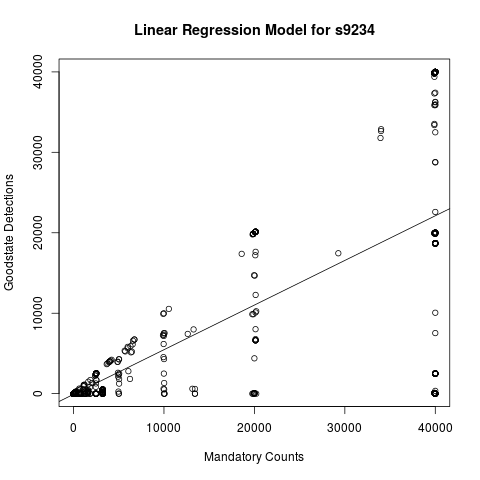
\includegraphics[scale=0.5]{Figures/s9234linereg.png}
    \end{figure}  

    The regression parameters for this model are: slope= 0.55 Intercept= -90.
    We can calculate the R-squared value by squaring $\rho$ from above, R-squared = 0.5929. 
    As was seen in the confusion matrix analysis, these values are strongly correlated, but not quite as strongly as we had hoped to see. 
    A take away from this is that while we can't really trust particular detections for circuit whose functions are unknown, we can predict about how important certain faults are relatively to one another.
    We can make this extrapolation because the regression analysis of this section is concentrated on the \textit{actual} mandatory counts, and goodstate observations.
    As opposed to the confusion matrix analysis which was only concerned about the presence of mandatory counts and goodstate observations.


    A similar analysis was performed on the DES56 circuit, and we again had more interesting results. 
    Pearson's correlation coefficient was calculated, $\rho = $ 0.88
    The linear lsregression model was plotted (Figure \ref{fig:deslinereg}).

    \begin{figure}[h!]
    \centering
    \caption{\label{fig:deslinereg}}
    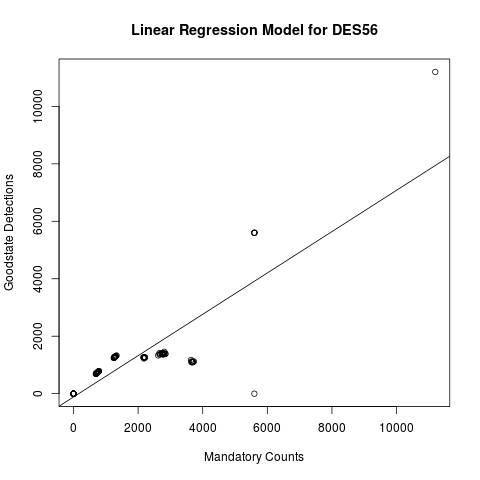
\includegraphics[scale=0.5]{Figures/deslinereg.png}
    \end{figure} 

    The regression parameters were calculated as: slope = 0.719, intercept = -116. 
    This time, we found a much higher R-squared value, which was 0.69.
    Again, we can see that when the functionality of a circuit is known, mandatory counts are a much better indicator of general fault importance. 

\section{conclusion}
    \label{sec:conc}
        \begin{comment}

    The prediction of fault importance will drastically shift the focus of most ATPG tools to allow for custom fault coverage levels. Another interesting possible application of this research is in regards to the estimation of fault coverage for parts of the circuit that are not tested using scan, but simply functional patterns. This latter application can apply to really any type of fault model not just cell-aware faults. In future work we plan to test the viability of this, and to also put safety bounds on how long we should run functional simulation, as well as testing this theory on other circuits and more extensively.  

    \end{comment}

    The cell-aware fault model is excellent at describing faults that could occur within standard cells. 
    But there is a very large number of cell aware faults in any one given circuit. 
    In order to more efficiently allocate testing resources during test, functional simulation with mandatory condition counters can be performed before hand. 
    This allows the tests engineers to more effectively target only those faults that are the most probable to cause errors during functional use. 
    The results of this paper also have some potential applications in intelligent speed-binning techniques. 
    To elaborate, you could test for wider and wider scopes of functionality, and speed-bin circuits more intelligently. 
    There are also potential applications of this methodology to artificially intelegent testing systems. 
    The results of this research are applicable to many different testing methodologies, and should not be restrictively thought of as cell-aware specific. 
    There is still much work to do in this area.
    We will likely proceed to test more circuits, and perform similar analysis.
    This will allow us to pinpoint more precisely what kinds of circuits these techniques are most effective against. 


    Using mandatory conditions for functional fault prediction has a wide variety of applications. 
    We presented the proper background material, and exhaustively detailed our proceedure as to make it easily repeatable. 
    We provided examples of mandatory condition calculations, and showed how they could be used to predict whether or not a cell-aware fault is functional.
    
\section{Acknowledgement}
    \label{sec:ack}
    TThe authors would like to thank Semiconductor Research Corporation who supports this research under Task ID 2465.001. The authors are also grateful for the support of our industrial liaisons. \\ 
\begin{center}
\textbf{Thank You}
\end{center}
\bibliographystyle{./IEEEtran}
\bibliography{./IEEEabrv,./cellAware}
\end{document}